\subsection{Helicopter model} \label{ssec:helimodel}

The helicopter model used is a nonlinear, six-degrees-of-freedom model of the Messerschmitt-Bölkow-Blohm Bo 105, developed by the NLR \cite{VanDerVorst2001}, modified with engine and rotor speed dynamics \cite{Gille2006}, and relevant structural and aerodynamic parameters taken directly from the Bo 105 flight manual \cite{BO105DataSheet}. The main rotor inflow is assumed to be uniform, with analytical blade element equations used for the forces and moments. The main rotor speed is dependant on the interplay between four sources of drag and the engine, the dynamics of which in turn are based on \cite{book:padfield} with reaction time modeled as a first-order lag. The tail rotor is modeled as an actuator disk, and linear aerodynamics are used to model the horizontal and vertical tails as well as the fuselage. The simulation model is run at 100Hz, assuming synchronous clean measurements and no turbulence. The state and action space of the model are given in Eq. \eqref{eq:heli_model_states} and Eq. \eqref{eq:heli_model_actions}.

\begin{equation} \label{eq:heli_model_states}
    s = \Big[u \enspace v \enspace w \enspace p \enspace q \enspace r \enspace \phi \enspace \theta\enspace \psi\enspace x\enspace y\enspace z\enspace \lambda_{0_{mr}}\enspace \lambda_{0_{tr}}\enspace \Omega \enspace P_{req}\enspace P_{av} \Big]^T
\end{equation}
\begin{equation} \label{eq:heli_model_actions}
    a = \begin{bmatrix} \delta_{col} & \delta_{lon} & \delta_{lat} & \delta_{ped} \end{bmatrix}^T
\end{equation}

Control inputs are given in percentages corresponding to how far that control input is between its minimum and maximum angle, with maximum being up or right, depending on the control channel. Because of phase lag inherent in rotorcraft, these control inputs do not correspond 1:1 with their respective control angles, as a certain degree of mixing occurs in the swashplate \cite{book:padfield}. The saturation limits of these control angles corresponding to 0\% and 100\% control input are given in Table \ref{tab:heli_control_ranges}. 

\begin{table}[ht]
    \centering
    \caption{Saturation limits of the control angles of the Bo 105 simulation model \cite{BO105DataSheet}}
    \label{tab:heli_control_ranges}
    \begin{tabular}{@{}lccc@{}}
    \toprule
    Control channel     & Symbol         & Associated control angle  & Saturation limits  \\ \midrule
    Collective          & $\delta_{col}$ & $\theta_0$        & [2, 18] deg   \\
    Longitudinal cyclic & $\delta_{lon}$ & $\theta_{1s}$     & [10, -5.5] deg \\
    Lateral cyclic      & $\delta_{lat}$ & $\theta_{1c}$     & [-6, 4] deg   \\
    Pedal               & $\delta_{ped}$ & $\theta_{0_{tr}}$ & [18, -6] deg  \\ \bottomrule
    \end{tabular}
\end{table}

\subsection{Flight controller} \label{ssec:controllerdesign}
The complete control system consists of a mixture of RL as well as conventional PID, and is shown in Fig. \ref{fig:controlsystem}. Only the longitudinal channels (collective and longitudinal cyclic) are controlled by the adaptive controllers, while the lateral channels (lateral cyclic and pedal) are controlled by conventional PID controllers. It must be noted that there is a strong degree of coupling between the different channels, and a unified controller would likely permit taking advantage of this in a way that multiple separate controllers cannot \cite{Enns2003a}. On the other hand, this set-up would also inevitably lead to slower learning, as it becomes inherently harder to learn the desired behaviour of multiple coupled states from a scalar reward signal. Although there is a strong degree of coupling between the different channels, the controllers have distinct enough tasks to allow for decoupling of the controllers. The resulting agent input states and action vectors are shown in Eq. \eqref{eq:state_loncol}. The state-selection and weight matrices required to extract these states from the complete state are given in Eqs. \eqref{eq:matrices_col} and \eqref{eq:matrices_lon}. A lower value for $Q^{col}$ is chosen to bring the magnitudes of the rewards of both agents more in line with each other, allowing for easier tuning.

\begin{figure}[ht]
    \centering
    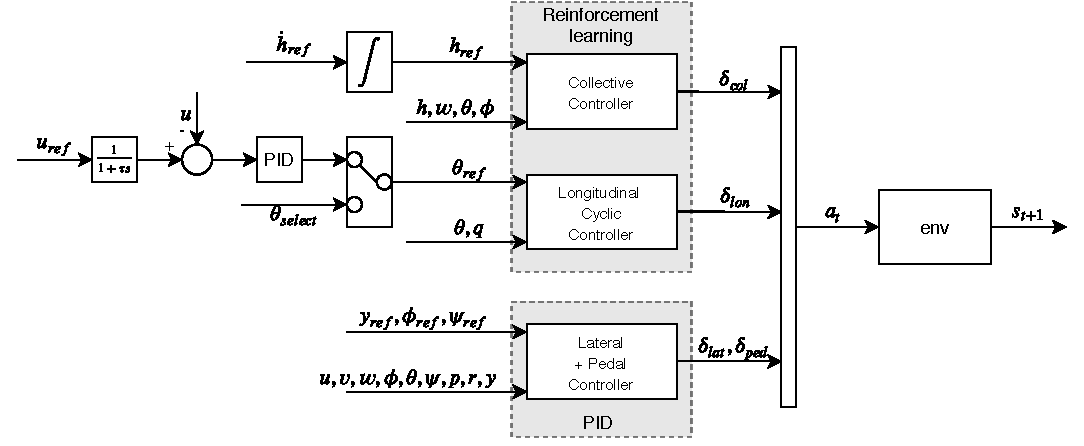
\includegraphics[width = 0.95\textwidth]{fig/3/controldiagram.pdf}
    \caption{High-level overview of the complete flight control system}
    \label{fig:controlsystem}
\end{figure}

\begin{equation} \label{eq:state_loncol}
    s^{col} = \begin{bmatrix} z & w & (z-z_{ref}) \end{bmatrix}^T \qquad s^{lon} = \begin{bmatrix} \theta & q & (\theta-\theta_{ref}) \end{bmatrix}^T
\end{equation}
\begin{equation} \label{eq:matrices_col}
    P^{col} = P^{lon} = \begin{bmatrix} 0 & 0 & 1 \end{bmatrix}
\end{equation}
\begin{equation} \label{eq:matrices_lon}
    Q^{col} = \begin{bmatrix} 0.1 \end{bmatrix} \quad Q^{lon} = \begin{bmatrix} 1 \end{bmatrix}
\end{equation}

\subsection{Hyperparameters} \label{ssec:hyperparameters}
The hyperparameters used by this implementation are shown in Table \ref{tab:hyperparams}. A number of these states have their values listed as *: these were determined empirically at first, but later fine-tuned by means a grid-search over multiple hyperparameter combinations as explained in Section \ref{ssec:trainingphase}. The others were determined empirically. The discount factor $\gamma$ is a measure of the importance of future rewards with respect to more immediate ones. As helicopter control generally does not have a very direct effect on the controlled states, a relatively large value of $\gamma$ is assumed. 

\begin{table}[]
    \centering
    \caption{Hyperparameters for the IDHP agents. The values indicated with an asterix were fine-tuned in the first part of the experiment}
    \label{tab:hyperparams}
    \begin{tabular}{@{}lll@{}}
\toprule
Parameter                         & Description                                        & Value              \\ \midrule
$\gamma$                          & Discount factor                                    & 0.8*               \\
$\sigma_w$                        & NN weight initialization standard deviation        & 0.1*               \\
$\tau$                            & Target critic mixing factor                        & 0.01*              \\
$\eta^{lon}_{a} \; \eta^{lon}_c$  & Longitudinal agent actor and critic learning rates & 5*                 \\
$\eta^{col}_{a} \; \eta^{col}_c$  & Collective agent actor and critic learning rates                    & 0.1*               \\
$\kappa$                          & RLS estimator forgetting factor                    & 0.999              \\
$\hat{F}_0, \hat{G}_0, \hat{P}_0$ & Initial RLS matrices                               & $I, 0, I\cdot10^8$ \\ \bottomrule
\end{tabular}
\end{table}